
\chapter{布拉格石人}
16世纪的时候,哈布斯堡王朝几乎控制着中欧的大部分地区,包括荷兰,西班牙以及西班牙在美洲的殖民地。
哈布斯堡王朝是第一个真正的世界霸主,每时每刻都能在它的某个统治区域内见到太阳,真正的日不落帝国。
它的统治者同时也是神圣罗马帝国皇帝,将权力中心放在布拉格。
十六世纪末期哈布斯堡王朝的鲁道夫二世皇帝,热衷于知识。他在艺术,科学(包括占星术和炼金术)和数学方面投入巨大精力,使布拉格成为世界的研究和学术中心。
因此,在这种浓厚的研究氛围中诞生了一个早期的机器人雏形,布拉格石人。

布拉格石人Golem(goh-lem)是一种粘土制成的机器人,在犹太传说中流传甚广。
石人有水火土构成。
在石人额头上刻上emet(希伯来语的“真相”),它就会被赋予生命。
石人虽然能够被真理激活,但却没有独立自主的意识,只能按照人们的指令行事。
幸好石人能令行禁止,因为他的力量非常强大,能够做到很多它的创造者所做不到的事情。
然而,它的绝对服从也有危险性,如不小心给他一些错误指示或因为其他一些意外事件可能会对它的铸造者带来不利影响。
石人力量强大但缺乏智慧。


在某些版本的石人传说中,石人是拉比.犹大为保卫布拉格犹太人想出的办法。
在16世纪中欧的许多地方,布拉格犹太人受到迫害。
拉比.犹大使用卡巴拉的秘密技术建造了石人,并用“真理”驱动它,来保卫布拉格的犹太人民。
但是并不是每个人都支持犹大的行为,担心会因为对生命力量的亵渎而产生意想不到的后果。
最终犹大被迫摧毁了石人,因为石人的蛮力最终导致了许多无辜生命的死亡。拉比.犹大将石人额头上的“emet”的第一个字母擦掉,就变成了“met”(希伯来语“死亡”),石人就被销毁了。

\section{统计学中的石人}
科学家也铸造了自己的石人。
只是这些石人很少有具体的物理形态,都是以计算机代码的形式存在于硅片上。
这些石人就是科学模型。
这些模型通过他们的预测能力以及对直觉的挑战或激发,来影响世界。
对“真理”的探求驱动着这些模型运转,但就像石人或现代机器人一样,科学模型既不是真也不是假,既不是先知也不是骗子。 
相反,它们是为某种目的而设计的结构。 这些结构非常强大,不知疲倦地按照编程逻辑进行计算。

\begin{figure}[htbp]
  \centering
 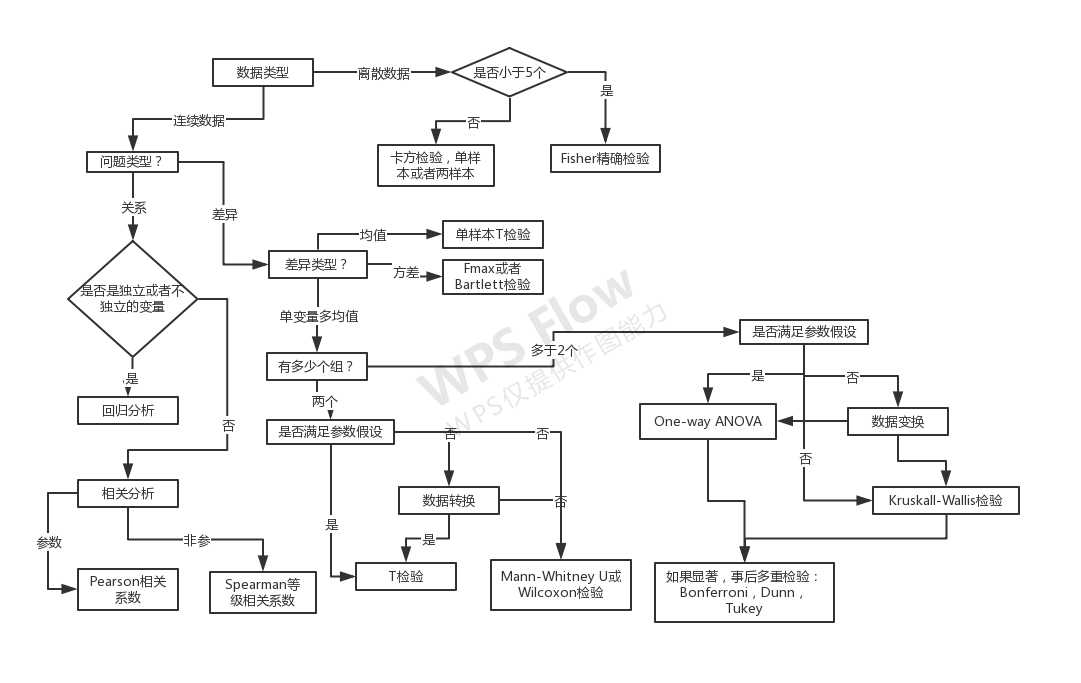
\includegraphics[width=0.9\textwidth]{chapters/figures/f1-1.png} 
 \caption{参数检验流程图}
\end{figure}

有时候这些逻辑也能发现一些设计师没想到的规律,这些规律可能有毫无意义也可能极具破坏性。
科学模型不是理想化的理性天使,而是强大的粘土机器人,他们没有自己的意识,
只会按照预设的短视指令笨手笨脚的工作。 
与拉比.犹大的石人一样,科学的"石人"也有它的好处和坏处。可以用但是会有风险。

统计模型有很多种。 每当有人部署一个简单的统计程序时,比如经典的t检验,她就会部署一个小石人。石人乖乖地进行精确计算,每次都以相同(接近)的方式执行,从不抱怨。 几乎每一个科学分支都会依赖于统计石人的探索能力。 在许多情况下,如果不使用模型,测量感兴趣的现象几乎是不可能的。 比如测量自然选择的强度或中微子的速度或亚马逊物种的数量,我们都必须使用模型。 模型是一个假肢,为我们做测量,并进行令人精确的计算,找到隐含的模式。

  然而,石人并没有智慧。 当所处的环境不适合其解答的时候,它也无法辨别。 它只知道自己的程序,没有别的。你告诉它怎么做就怎么做。所以统计科学能够一直发展下去,也有赖于有许多不同的石人,每个石人都只在特定的场景下有用。 从这个角度来看,统计既不是数学也不是科学,而是工程学的一个分支。 和工程学一样,一套通用的设计准则产生了各种各样的特定应用。

  这种多样化的应用解释了为什么统计课程经常让初学者感觉非常混乱。 因为没有一个统一的方法去建立、完善和评价统计模型,大家拿到的是一大堆叫做“测试”的石人,每项“测试”都有特定的目的。 像如图1.1中的决策树,就很常见。 通过回答一系列问题,用户可以根据他们的研究的环境选择所谓的“正确”方法。

  虽然经验丰富的统计学家能够掌握这些统计工具的统一性,但学生和研究人员很少能达到这样的深度。高级统计课程确实强调工程原理,但大多数科学家达不到这样的标准。 这种方式的统计学教学有点像逆向教学法,从桥梁建设开始学逐步深入到基础物理学。 因此,学生和许多科学家倾向于使用图1.1之类的图表既不不深入考虑他们的原理结构,也不深究每个工具所代表的模型,也没有任何框架来帮助他们在真正的研究过程中做一些权衡。 当然这样做也没错。

  对于一些人来说,预制的石人工具箱就是他们所需要的。 只要保证在经过充分测试的上下文环境中使用,在适当的任务中仅使用少数几个不同的程序,就可以完成许多优秀的科学研究。 这类似于大多数水管可能并不了解流体动力学,但他依然可以完成大量的工作。 但是当研究人员进行创新研究,突破他们专业的界限时,就有问题了。 这就好比让水管工提升为液压工程师。

  为什么统计测试不足以支持创新研究呢? 描述性统计 的经典方法往往缺乏灵活性并且很脆弱。缺乏灵活性,意思是当聚焦到非常具体的研究问题时,他们有非常有限的方式来适应。脆弱的意思是在应对新的问题时,经典的统计工具往往很失败。这很重要,因为在大多数科学边界,几乎没有哪个清楚哪种程序适合。在新的研究问题中,没有一个传统的石人被评估过,因此很难选择一个然后去了解它的行为方式。Fisher精确检验就是一个很好的例子,它的应用面实际非常窄。但只要细胞数量很少,人们就会经常使用它。我已经在科学期刊上亲自阅读了Fisher精确测试的数百种用途,但除了Fisher最初的使用环境之外,我从未见过正确的使用方法。甚至像最普通的线性回归这样的方法,虽然在许多方面都非常灵活,能够处理大量有趣的假设,有时也很脆弱。比如,如果预测变量存在大量测量误差,线性回归就极有可能失败。更重要的一点,其他有些方法几乎总是可以做得比普通的线性回归好,但主要是因为过度拟合的原因(第6章)。

  问题的关键不在于这些统计工具是否专业,它们当然很专业。 关键问题是这些经典的工具连许多常见的研究问题都处理不了。 每个活跃的科学领域都会面临特定的测量和解释困难,与其他领域的其他科学家的理论交流用的几乎都是别人无法理解的“黑话”。统计专家是可以提供帮助,但由于缺乏对该学科的经验和理论,经常解释的驴唇不对马嘴。 在这样的环境下,预制的石人根本没有任何用处。 更糟糕的是,这些石人还会把大本营布拉格摧毁。 而如果我们不断添加新类型的工具,很快就没法维护了。

  相反,研究人员需要的是一些统一化的构建石人的工程理论,一套设计、建立和完善统计程序的设计原则。 统计哲学的每个主要分支都拥有这样一个统一理论。 但是这个理论从不在介绍性课程中讲授 - 甚至在高级课程中也没有。 所以,最好将统计推断重新定位为一组策略,而不是一组工具。
